% \section{Sémantique concrète pour un langage assembleur}
\itodo{Relire et checker la cohérence de la notation en expressions}

Dans ce chapitre nous proposons un modèle simplifié pour le langage assembleur et une sémantique concrète pour ce langage.

Lors de l'analyse d'un binaire, il est crucial de pouvoir analyser chaque instruction.
La question centrale est la suivante : quelle est l'opération réalisée par cette instruction ?
En particulier quels sont ses opérandes en entrées, en sortie, et comment sont-ils lus et modifiés ?
Prenons l'instruction \texttt{push ecx}. 
Il est clair que le registre \ecx\ est un opérande mais cette information est insuffisante : cette instruction consiste à empiler la valeur de \ecx\ sur la pile, elle modifie donc le pointeur de pile \esp\ et écrit à une adresse mémoire.

Nous reprenons la classification informelle en trois niveaux d'information proposée par Calvet \cite{Calvet2013} à la figure \ref{fig:niveaux_sem}, par exemple pour l'instruction \texttt{push ecx} :
\begin{itemize}
 \item Niveau 1 - Opérandes explicites : \ecx
 \item Niveau 2 - Opérandes implicites précis : \ecx\ et \esp\ sont des entrées, l'adresse mémoire à l'adresse $esp-4$ est une sortie
 \item Niveau 3 - Opération : l'instruction décrémente \esp\ de 4 puis écrit à l'adresse mémoire pointée par \esp\ la valeur qui est dans \ecx
\end{itemize}

\begin{figure}
\begin{center}
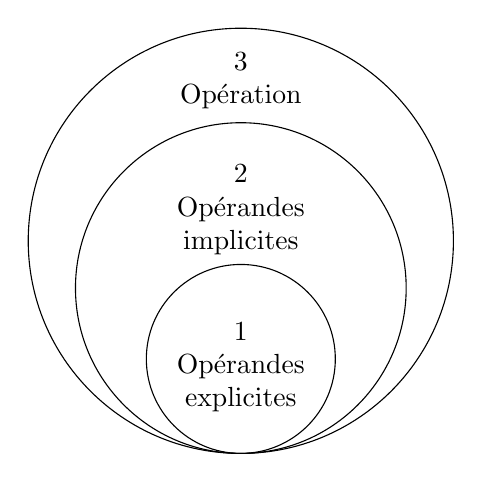
\begin{tikzpicture}[text centered]
% Definition of circles
\colorlet{circle edge}{black!100}
\colorlet{circle area}{black!20}

\tikzset{filled/.style={fill=circle area, draw=circle edge, thick},
    outline/.style={draw=circle edge, thick}}
    \draw (0, -1) arc (-90:270:2.7cm) node[above=4.25cm, text width=4cm]{3\\Opération};
    \draw (0, -1) arc (-90:270:2.1cm) node[above=2.4cm, text width=4cm]{2\\Opérandes\\implicites};
    \draw (0, -1) arc (-90:270:1.2cm) node[above=0.4cm, text width=4cm]{1\\Opérandes\\explicites};
%     \node[anchor=south] at (current bounding box.north) {Progwramme};
\end{tikzpicture}
\end{center}
\caption{Niveau des précision des informations sur une instruction}
\label{fig:niveaux_sem}
\end{figure}

Une sémantique concrète se place au niveau 3 : elle donne une information exhaustive sur l'opération réalisée par chaque instruction.
Ce chapitre sera donc consacré à la définition d'une sémantique concrète pour un langage assembleur simplifié.
Nous verrons par la suite que pour certaines analyses une sémantique de niveau 2 peut-être suffisante.

\section{Sémantique concrète pour un langage assembleur}
\paragraph{Représentation de la mémoire et des registres.}
On peut voir la mémoire comme un tableau contenant la pile et le tas, indexés sur les entiers. Les registres sont des variables distinctes de la mémoire et sont en nombre limité.
L'assembleur distingue plusieurs modes d'adressage dont les deux principaux sont l'adressage direct et indirect : à l'exécution \eax\ prend la valeur du registre \eax\ (adressage direct) tandis que \texttt{[eax]} fait référence à la valeur en mémoire à l'adresse contenue dans \eax\ (adressage indirect).
Ces éléments sont définis formellement à la définition \ref{def:sem_conc_var}.

% \begin{rem}
%  Avec cette définition, une valeur en mémoire peut pointer vers un registre. De même un registre peut pointer vers un autre registre.
%  Ces deux possibilités ne sont pas réalisables avec l'assembleur \xq\ ou \xs.
% \end{rem}


% \begin{defi}
% On définit les symboles $x\in\BX$ comme constitués de variables $v\in\BV$ et de pointeurs $p\in\BP$ vers des variables. $\BV$ contient un ensemble fini de registres $a\in\BA$ et un tableau de taille finie $\BT=\textlbrackdbl 0,\ T\textrbrackdbl$. Les éléments de $\BP$ sont des pointeurs vers une variable : $\{[v],\ v\in \BV\}$.
% Les valeurs possibles pour les variables sont dans $\BN$.
% \label{def:sem_conc_var}
% \end{defi}

\begin{defi}
On définit un ensemble fini de registres $a\in\BA$ et un tableau de taille finie $\BT=\{T_n,\ n\in\textlbrackdbl 0,\ N\textrbrackdbl\}$. Les variables sont soit un registre soit dans le tableau : $\BV=\BA\cup\BT$.
% On définit un symbole $x\in\BX$ à partir d'une variable $v\in\BV$ comme étant soit une variable sous un mode d'adressage direct, représentée $v$, soit une variable sous un mode d'adressage indirect, notée $[v]$. On note $\BP$ l'ensemble des variables sous un adressage indirect : $\BX=\BV\cup\BP$.
Les expressions $\BE$ sont de l'un des types suivants :\\
% $empl:=$ $a\in\BA$ $|$ $T_n$ avec $n\in\BT$ $|$ $[v]$ avec $v\in\BA\cup\BT$ \\
$expr:=$ $\bot$ $|$ $n\in\BN$ $|$ $a\in\BA$ $|$ $T_n$ avec $n\in\BN$ $|$ $[a]$ avec $a\in\BA$ $|$ $[T_n]$ avec $n\in\BN$
% Les valeurs possibles pour les variables sont dans $\BN$.
\label{def:sem_conc_var}
\end{defi}

% \begin{defi}
% On définit deux opérateurs. Le premier, $T$, permet d'accéder à la mémoire et s'applique à $T: \BT=\textlbrackdbl 0,\ N\textrbrackdbl$.\\
% $expr:= v\in\BV$ $|$ $[v]$ avec $v\in\BV$ $|$ $T(n)$ avec $n\in\BT=\textlbrackdbl 0,\ N\textrbrackdbl$
% \label{def:operateurs_expressions}
% \end{defi}

\paragraph{Langage assembleur simplifié.} Nous allons définir un langage intermédiaire dans lequel on peut transcrire chaque instruction \xq\ en une liste d'instructions atomiques de notre langage simplifié.
Les instructions \xq\ sont disponibles à différentes adresses entières. 
Les instructions atomiques sont de plusieurs type explicités en définition \ref{def:sem_instructions} : le premier consiste en l'assignation.
Il est possible d'assigner un symbole ou une combinaison de symboles (à l'aide d'une fonction sur les entiers) à un symbole. 
Le second type d'instruction regroupe les sauts inconditionnels et conditionnels.
On distingue également l'instruction \texttt{end} forçant l'arrêt du programme.

\begin{defi}
Les instructions atomiques d'un programme sont de ce type, quelle que soit la fonction totale g de $\BN^m$ dans $\BN$ avec $x$, $x'$ et $x_i$ étant des expressions.\\
$inst:=\ $\emph{$x\leftarrow g(x_1, ..., x_m)$ $|$ goto $x$ $|$ if $x$ then $goto\ x'$ $|$ end}
\label{def:sem_instructions}
\end{defi}


% \paragraph{Exemples naïfs de la représentation d'instructions assembleur \xq.}
La figure \ref{fig:sem_exemples_insts} donne des exemples de transcription d'instructions \xq\ dans le langage défini précédemment. 
Ils sont naïfs au sens que les instructions \xq\ sont plus complexes et un simple \sub\ provoque des effets de bord modifiant des registres. Ce point sera développé par la suite lorsque nous discuterons des implémentations possibles pour cette sémantique concrète.
\\

\begin{figure}
 \begin{center}
  \begin{tabular}{|l|l|}
   \hline
   Instruction \xq & Instructions atomiques équivalentes\\
   \hline
   mov eax, 3 & $eax\leftarrow 3$ \\
   \hline
   mov [eax], 4 & $[eax]\leftarrow 4$ \\
   \hline
   mov [eax+1], 5 & $tmp\leftarrow addition(eax, 1)$ \\
    & $[tmp]\leftarrow 5$ \\
   \hline
   jmp eax & $goto\ eax$ \\
   \hline
   sub eax, 3 & $eax\leftarrow soustraction(eax, 3)$ \\
   \hline
  \end{tabular}
 \end{center}
\caption{Exemple de transcription d'instructions \xq\ dans le langage assembleur simplifié}
\label{fig:sem_exemples_insts}
\end{figure}


Comme nous avons vu dans les parties précédentes, un programme est simplement composé d'un ou plusieurs blocs d'octets à charger en mémoire. Une fois ces segments chargés dans le tableau $\BT$ représentant la mémoire, le point d'entrée du programme est placé dans le registre \texttt{ep}.


% \begin{defi}
% L'adresse 
% \label{def:sem_programme}
% \end{defi}

% 
%On note $\PMN$ l'ensemble des parties de $\BN$ de taille inférieure ou égale à M $\in\BN$ en excluant l'ensemble vide (représenté par $\bot$).

Pour faire le lien entre la machine et les instructions exécutées, il est nécessaire de pouvoir désassembler des instructions en mémoire. C'est le rôle de l'opérateur de désassemblage (définition \ref{def:sem_desassembleur}).

\begin{defi}
% On appelle $D$ l'opérateur de désassemblage qui à une adresse de la mémoire $\BT$ associe une instruction et la taille de cette instruction dans $\BN$. \\
On appelle $D$ l'opérateur de désassemblage qui à une adresse de la mémoire $\BT$ associe une liste d'instructions atomiques et la taille de cette instruction dans $\BN$. \\
Pour toute adresse $t\in\BT$, on note $D(t)=d_1..d_n$ et $D_S(t)$ respectivement la suite d'instructions atomiques à l'adresse $t$ et la taille de cette instruction.\\
Dans le cas où il n'y a pas d'instruction valide à l'adresse $t$, $D(t)=\bot$ et $D_S(t)=0$.
\label{def:sem_desassembleur}
\end{defi}

Une sémantique concrète cherche à définir les opérations de chaque instruction de la manière la plus précise qu'il soit afin de pouvoir simuler une exécution réelle du programme.
Pour cela on va utiliser un store qui conserve l'état des variables lors de l'exécution du programme.
Toute variable non initialisée a la valeur spéciale $\bot$ tandis que les variables définies ont des valeurs entières (définition \ref{sem_store_dynamique}).

\begin{defi}
 Un store dynamique $\Theta$ associe à chaque variable une valeur, $\Theta:\BV\rightarrow\BN\cup\{\bot\}$.\\
 Si v est une variable et n une valeur dans $\BN\cup\{\bot\}$, on note $\Theta[v\leftarrow n]$ l'assignation de v à n dans $\Theta$.
\label{sem_store_dynamique}
\end{defi}

Pour permettre l'adressage indirect on doit également définir le store sur l'ensemble des symboles de la forme $[v]$.
La définition \ref{sem_store_dynamique_pointeurs} étend la notion de store à l'adressage indirect afin que chaque symbole ait une valeur.


\begin{defi}
 Définissons une extension $\Theta_X$ d'un store $\Theta : \BV\rightarrow\BN\cup\{\bot\}$ à $\BE\rightarrow\BN\cup\{\bot\}$. Soit $x\in\BX$.
 \begin{itemize}
  \item Si $x=\bot$, $\Theta_X(x)=\bot$
  \item Si $x\in\BN$, $\Theta_X(x)=n$
  \item Si $x\in\BV$ : $\Theta_X(x)=\Theta(x)$
  \item Sinon, $x=\textlbrackdbl v\textrbrackdbl$ avec $v\in\BV$.
  \begin{itemize}
   \item Si $\Theta(v)=\bot$ alors $\Theta_X(x)=\bot$
   \item Si $\Theta(v)\in\BN$ et $\Theta(v)\notin\textlbrackdbl 0,\ N\textrbrackdbl$ alors $\Theta_X(x)=\bot$
   \item Sinon $\Theta(v)\in\BN$ et $\Theta(v)\in\textlbrackdbl 0,\ N\textrbrackdbl$, alors $\Theta_X(x)=\Theta(\Theta(v))$.
  \end{itemize}
 \end{itemize}
  De même on étend l'opération d'assignation d'une valeur à une expression de la manière suivante. Soit $x\in\BE$ et $n\in\BN\cup\{\bot\}$.
  \begin{itemize}
  \item Si $x=\bot$, $\Theta_X[x\leftarrow n]$ n'a aucun effet
  \item Si $x\in\BN$, $\Theta_X[x\leftarrow n]$ n'a aucun effet
  \item Si $x\in\BV$ : $\Theta_X[x\leftarrow n]$ est équivalent à $\Theta[x\leftarrow n]$.
  \item Sinon, $x=\textlbrackdbl v\textrbrackdbl$ avec $v\in\BV$.
    \begin{itemize}
   \item Si $\Theta(v)=\bot$ alors l'assignation n'a aucun effet
   \item Si $\Theta(v)\in\BN$ et $\Theta(v)\notin\textlbrackdbl 0,\ N\textrbrackdbl$ alors l'assignation n'a aucun effet
   \item Sinon $\Theta(v)\in\BN$ et $\Theta(v)\in\textlbrackdbl 0,\ N\textrbrackdbl$, alors $\Theta_X[x\leftarrow n]$ se résoud par $\Theta[T_{\Theta(v)}\leftarrow n]$.
  \end{itemize}
  \end{itemize}
\label{sem_store_dynamique_pointeurs}
\end{defi}

\paragraph{Règles de transition.}
Les états d'exécution sont de la forme \textlangle$t, \Theta_X$\textrangle\ où $t$ est une adresse ou l'adresse invalide (ou finale) $\bot$. 
À chaque instruction exécutée, il y a une transition \textlangle$t, \Theta_X$\textrangle$\rightarrow$\textlangle$t', \Theta_X'$\textrangle.\\
Si il y a une suite de transitions amenant d'un état \textlangle$t, \Theta_X$\textrangle\ à l'état \textlangle$t', \Theta_X'$\textrangle, on note \textlangle$t, \Theta$\textrangle$\rightarrow^*$\textlangle$t', \Theta_X'$\textrangle.\\
Un programme s'arrête en partant de l'état initial \textlangle$ep, \Theta_X$\textrangle\ où \texttt{ep} est son point d'entrée si et seulement si \textlangle$ep, \Theta_X$\textrangle$\rightarrow^*$\textlangle$\bot, \Theta_X'$\textrangle. 
Le programme dans ce cas s'arrête à la première occurrence d'une adresse finale ou invalide $\bot$.

On définit par la suite la sémantique des instructions atomiques et on étend donc les états d'exécution à celles-ci : on note \textlangle$t:d_1..d_n, \Theta_X$\textrangle\ l'état \textlangle$t, \Theta_X$\textrangle\ sur lequel il y a les instructions atomiques $d_1..d_n$ à évaluer.
À partir d'un état \textlangle$t, \Theta_X$\textrangle, on commence par déterminer les instructions atomiques à évaluer à l'aide de l'opérateur de désassemblage : on arrive à un état \textlangle$t:D(t), \Theta_X$\textrangle=\textlangle$t:d_1..d_n, \Theta_X$\textrangle\ dans lequel on va pouvoir évaluer les instructions atomiques l'une après l'autre. 
Une fois que toutes ces instructions ont été évaluées et si aucune d'elle n'a provoqué de saut vers une adresse différente, on passe à l'instruction qui suit séquentiellement à l'adresse $t+D_S(t$\textrangle.

L'état initial du store est : $\forall v\in\BV, \Theta_X(v)=\bot$ et l'on part du point d'entrée \texttt{ep}. Les règles de transition suivantes permettent d'aboutir à une adresse finale ou invalide $\bot$ si le programme termine.

% \begin{tabbing}
% \textlangle$t:x\leftarrow g(x_1, ..., x_m),\ \Theta_X$\textrangle\ \=$ \longrightarrow $ \textlangle$t+D_S(t),\ \Theta_X[x\leftarrow\bot]$\textrangle~~~~~~~~~~~~~~~~~~~~~~~~~~~~~~~\=si $\exists i, \Theta_X(b_i)=\bot$\\
%                                                                    \>$ \longrightarrow $ \textlangle$t+D_S(t),\ \Theta_X[x\leftarrow g(\Theta_X(b_1),...,\ \Theta_X(b_m))]$\textrangle \> sinon\\ \\
% 
% \textlangle$t:goto\ x,\ \Theta_X$\textrangle\>$\longrightarrow $ \textlangle$\Theta_X(x),\ \Theta_X$\textrangle\> \\ \\
% 
%  \textlangle$t:if\ x\ then\ goto\ x',\ \Theta_X$\textrangle\>$ \longrightarrow $ \textlangle$\Theta_X(x'),\ \Theta_X$\textrangle\ \>si $\Theta_X(x)=1$\\
% 									    \>$ \longrightarrow $ \textlangle$ t+D_S(t),\ \Theta_X$\textrangle\ \>sinon\\ \\
% 
% \textlangle$t\notin\BT,\ \Theta_X$\textrangle\>$ \longrightarrow $ \textlangle$\bot,\ \Theta_X$\textrangle\\
% \textlangle$t:end,\ \Theta_X$\textrangle\>$ \longrightarrow $ \textlangle$\bot,\ \Theta_X$\textrangle
% \end{tabbing}


\begin{center}
\begin{tabular}{lcl}
% \hline
\textlangle$t\in\BT;\ \Theta_X$\textrangle & $\longrightarrow$ & \textlangle$t:D(t);\ \Theta_X$\textrangle  \\
& & \\
% \hline
\textlangle$t:x\leftarrow g(x_1, ..., x_m), d_2..d_n;\ \Theta_X$\textrangle & $\longrightarrow$  & \textlangle$t:d_2..d_n;\ \Theta_X[x\leftarrow\bot]$\textrangle\  \\
 &   & ~~~si $\exists i, \Theta_X(x_i)=\bot$  \\
 & $\longrightarrow$  & \textlangle$t:d_2..d_n;\ \Theta_X[x\leftarrow g(\Theta_X(x_1),...,\ \Theta_X(x_m))]$\textrangle\    \\
  &   & ~~~sinon  \\
% \hline
& & \\
\textlangle$t:goto\ x, d_2..d_n;\ \Theta_X$\textrangle & $\longrightarrow$ & \textlangle$\Theta_X(x);\ \Theta_X$\textrangle  \\
% \hline
& & \\
\textlangle$t:if\ x\ then\ goto\ x',\ \Theta_X$\textrangle\ & $\longrightarrow$ & \textlangle$\Theta_X(x'),\ \Theta_X$\textrangle\\\
  &   & ~~~si $\Theta_X(x)=1$  \\
 & $\longrightarrow$ & \textlangle$ t+D_S(t),\ \Theta_X$\textrangle\\
   &   & ~~~sinon  \\
% \hline
& & \\
\textlangle$t:end, d_2..d_n;\ \Theta_X$\textrangle\ & $\longrightarrow$ & \textlangle$\bot;\ \Theta_X$\textrangle  \\
% \hline
& & \\
\textlangle$t:\bot;\ \Theta_X$\textrangle\ & $\longrightarrow$ & \textlangle$\bot;\ \Theta_X$\textrangle  \\
% \hline
& & \\
\textlangle$t\in\BT:\emptyset;\ \Theta_X$\textrangle & $\longrightarrow$ & \textlangle$t+D_S(t);\ \Theta_X$\textrangle  \\
& & \\
\textlangle$t\notin\BT;\ \Theta_X$\textrangle\ & $\longrightarrow$ & \textlangle$\bot;\ \Theta_X$\textrangle  \\
% \hline
\end{tabular}
\end{center}

\itodo{est-il possible de mettre $\bot$ dans une variable ? -> c'est une erreur plutôt non ?}

Dans la suite nous appellerons évaluation sémantique ou \texttt{sem\_eval} la fonction qui, à une adresse $t$ et un store $\Theta_X$, associe l'état sur les instructions \xq\ suivant : si $t'$ et $\Theta_X'$ sont les premières valeurs vérifiant \textlangle$t, \Theta$\textrangle$\rightarrow^*$\textlangle$t', \Theta_X'$\textrangle\ avec $t\ne t'$ alors \texttt{sem\_eval}$(t, \Theta_X)=(t', \Theta_X')$.


\section{Assembleur et langage intermédiaire}
En pratique pour analyser un programme assembleur on veut en avoir une représentation dont on connaît la sémantique concrète.
On va pour cela réécrire le programme dans un langage intermédiaire et effectuer les analyses sur le programme en langage intermédiaire.
Le langage défini dans ce chapitre est un langage intermédiaire possible.

Une des difficultés rencontrées dans la transformation d'un langage assembleur en langage intermédiaire est la richesse sémantique du langage \xq\ qui contient des centaines d'instructions et utilise de nombreux registres et drapeaux du processeur.
L'instruction \texttt{sub eax, b} par exemple soustrait l'opérande \texttt{b} à \eax\  en stockant le résultat de l'opérant dans \eax.
Le mnémonique \texttt{sub} désigne une vingtaine de variantes de la soustraction selon la taille des opérandes pris en compte. Elle effectue l'opération \texttt{eax-b} et met à jour les drapeaux CF et OF indiquant un dépassement de valeur entière, le drapeau de signe SF, le drapeau ZF (à 1 si le résultat est nul) et celui de parité PF.

Une instruction assembleur va donc être traduite en une ou plusieurs instructions atomiques dans le langage intermédiaire, que l'on sait équivalentes sémantiquement à l'instruction \xq\ et dont on a une sémantique concrète pour les exécuter.
Une difficulté pratique vient de la richesse du langage \xq\ : écrire l'équivalence de chacun de ses instructions dans le langage intermédiaire choisi est une tâche longue et prône aux erreurs, notamment lors de l'analyse de la documentation. 
Pour cette raison nous avons rapidement choisi de nous orienter vers des langages intermédiaire pour lesquels cette étape a déjà été réalisée.

\section{Revue de littérature des langages intermédiaires}
\todo[inline]{Jakstab: \\
TraceSurfer: \\
Renovo : \\
LLVM : \\
Implem en C: \\
TraceSurfer: \\
Pin : \\
Xed : \\
}


Parmis les projets de langages intermédiaires existants et fournissant d'une part une transcription depuis l'assembleur et d'autre part une sémantique concrète du langage considéré, nous nous sommes intéressés à BAP \cite{BAP11}. 
BAP est le successeur du projet BitBlaze qui a défini et développé une plateforme d'analyse statique basée sur le langage intermédiaire Vine IL \cite{bitblaze08}. 
Sémantiquement le langage intermédiaire défini par BAP ne diffère pas fondamentalement de celui défini dans ce chapitre. 
Ils définissent également un opérateur permettant de gérer l'adressage indirect : \texttt{load($e_1$, $e_2$, $e_3$, $\tau_{reg}$)} place la valeur de l'expression $e_1$ à l'adresse $e_2$, ainsi \texttt{load($x$, $eax$, $e_3$, $\tau_{reg}$)} effectue l'opération \texttt{$[eax]\leftarrow x$}. 
Le paramètre $e_3$ a une valeur booléenne indiquant si la machine fonctionne en petit ou grand boutiste et $\tau_{reg}$ indique le nombre d'octets qui doivent être copiés. 
L'avantage de BAP par rapport au langage présenté précédemment est qu'il est est bien plus proche du langage assembleur : les valeurs des variables ne sont pas dans $\BN$ mais dans $\textlbrackdbl 0,\ 2^{32}-1\textrbrackdbl$, $\textlbrackdbl -2^{31},\ 2^{31}-1\textrbrackdbl$, $\textlbrackdbl 0,\ 2^{64}-1\textrbrackdbl$ ou $\textlbrackdbl -2^{63},\ 2^{63}-1\textrbrackdbl$ selon la machine que l'on cherche à modéliser et le type des variables (signé ou non). 
De même les fonctions entières sont explicitées et contiennent, entre autres, des opérations binaires comme l'addition, le ``ou'' logique, la comparaison de deux valeurs.


\section{Langage intermédiaire et analyse de binaires}
Un programme sous forme d'instructions dans un langage intermédiaire est plus facile à exploiter qu'un programme assembleur puisqu'on a une sémantique concrète clairement définie et assez compacte.
Il est donc, comme nous le verrons par la suite, fréquent de construire des méthodes de désassemblage et d'analyse de binaires autour d'une représentation intermédiaire.

\paragraph{Approche globale.}
Une première approche consiste, à l'instar de la compilation, à transformer l'intégralité du programme assembleur en un programme en langage intermédiaire et à effectuer les analyses sur cette représentation intermédiaire.
Cette approche est illustrée par le graphique donné à la figure \ref{fig:diag_approche_globale}. La partie d'analyse consiste en l'exécution ou l'émulation du programme dans son langage intermédiaire en partant du point d'entrée.
Une première instruction est décodée, analysée et ajoutée dans le graphe de flot de contrôle du programme. Puis cette instruction est évaluée selon la méthode d'évaluation sémantique précédemment définie.
Cette évaluation a des conséquence sur l'état interne du processeur et de la mémoire de la machine réelle ou virtuelle (selon si l'analyse est réalisée par exécution\todo{exécution ? alors qu'on ne parle que d'émulation/store ?} ou émulation).
L'instruction qui doit être exécutée ensuite est cette présente à l'adresse donnée par le registre d'exécution (\eip\ en assembleur \xq). On récupère alors cette instruction pour l'analyser à son tour.

\begin{figure}
\begin{center}
\scalebox{1}{
\begin{tikzpicture}[->,scale=1,>=stealth',thick]
\node[state] (BIN){Binaire};
\node[state, right=1.4cm  of BIN] (ASM){ASM};
\node[state, right=1.4cm of ASM] (IR){LI};
\node[state, right=6cm of IR] (INST){Instruction};    
\node[state, above=1cm of INST.north] (CFG){CFG};
\node[state, rectangle split, rectangle split parts=2, draw, below left=1.5cm and -0.5cm of INST, label=État interne, text width=2cm] (ETAT_MEM){Registres \nodepart{second} Mémoire};

\draw (BIN) --  node[above=0.5cm]{\small Désassemblage} (ASM);-1
\draw (ASM) -- node[above=0.5cm]{\small Transcodage} (IR);
\draw (IR) -- node[above]{Décodage} (INST);
\draw (INST) -- node[right=.2cm]{Ajout} (CFG);
\draw ($(ETAT_MEM.north west) + (0, -.4) $)  -| node[above right=.0cm and 0.4cm, text width=4cm](LEC){Lecture de la \\prochaine instruction} (IR);
\draw (INST) |- node[above right=0.3cm and .0cm, text width=4cm](EVAL){Évaluation \\sémantique} ($ (ETAT_MEM.north east) + (0,-.4) $);
\draw (INST) |- ($ (ETAT_MEM.south east) + (0,.35) $);

\node [fit={($ (LEC.west) + (0.20,0) $) ($(ETAT_MEM.south) + (0, +0)$) (INST) ($(CFG.north) + (0, 0.0)$) ($ (EVAL) + (0,0) $)}, draw, label=\large Analyse] {};
\end{tikzpicture}
}
\end{center}
\caption{Approche globale de l'analyse de binaires à l'aide d'un langage intermédiaire}
\label{fig:diag_approche_globale}
\end{figure}


Le souci de cette approche est qu'elle induit des potentielles pertes d'informations : la représentation d'origine du binaire sous forme d'octets n'est plus accessible dans la représentation intermédiaire.
Pourtant on ne peut pas séparer les instructions de leur représentation en mémoire : si une instruction est codée à l'adresse \adr{a} sur deux octets et que l'octet à l'adresse \adr{a+1} est modifié, cette modification peut être transcrite dans le langage intermédiaire mais il est toujours nécessaire de connaître l'octet à l'adresse \adr{a} pour pouvoir décoder la nouvelle instruction.

La figure \ref{fig:prg_asm_li} donne un exemple de ce cas. Le segment de code donné est constitué de trois instructions dont l'une modifie la valeur du registre \edi. Supposons que le but de l'analyse est de connaître la valeur de \edi\ à l'issue de l'exécution.
Les deux premières instructions servent à modifier le second octet de l'instruction modifiant \edi\ de \texttt{01} à \texttt{02} transformant cette instruction en \texttt{mov edi, 2}.
L'approche globale de la transcription du programme dans le langage intermédiaire, bien que chaque instruction assembleur soit sémantiquement équivalente aux instructions transcrites, résulte en un programme qui n'est pas auto-modifiant. Il est composé des quatre instructions de la dernière colonne du tableau.
Les trois premières écrivent la valeur 2 en mémoire à l'adresse \adr{0x804806c} et la dernière, indépendante, attribue la valeur 1 au registre \edi.
Ainsi l'analyse conclurait, à tort, que l'exécution du segment de code assembleur d'origine attribue 1 à \edi, au lieu de 2.

Ainsi, pour pouvoir utiliser ce langage intermédiaire dans le cas d'un programme auto-modifiant, il est nécessaire d'avoir accès à une représentation en mémoire du binaire exécuté lors de son exécution sous forme intermédiaire.

\begin{figure}
\begin{center}
\begin{tabular}[b]{|l|l|l|l|}
\hline
Adresse & Octets & Instruction ASM & Transcription en LI\\ 
\hline
 8048060  &  b8 6b 80 04 08         &  mov    eax,0x804806b & eax $\leftarrow$ 0x804806b\\
 8048065  &  66 c7 40 01 02 00      &  mov    [eax+1], 2 & tmp $\leftarrow$ addition(eax, 1)\\
          &                         &                                & [tmp] $\leftarrow$ 2 \\
 804806b  &  bf 01 00 00 00         &  mov    edi, 1 & edi $\leftarrow$ 1 \\
\hline
\end{tabular}
\end{center}
\caption{Programme assembleur et sa transcription dans le langage intermédiaire}
\label{fig:prg_asm_li}
\end{figure}

% \begin{figure}
% \begin{tabular}[b]{|l|l|l|}
% \hline
% Adresse & Octets & Instruction\\ 
% \hline
%  8048060  &  b8 6b 80 04 08         &  mov    eax,0x804806b \\
%  8048065  &  66 c7 40 01 02 00      &  mov    WORD PTR [eax+0x1],0x2 \\
%  804806b  &  bf 01 00 00 00         &  mov    edi,0x1 \\
%  8048070  &  c3                     &  ret     \\
% \hline
% \end{tabular}
% \caption{Programme transcrit dans le langage intermédiaire}
% \label{fig:prg_li}
% \end{figure}



\paragraph{Approche atomique.}
En pratique nous souhaitons donc avoir accès à la représentation sous forme binaire du programme intial.
Nous allons donc commencer par le charger en mémoire comme une partie intégrante de l'état interne de la machine.
C'est le comportement attendu d'une machine de Harvard modifiée \todo{von neumann?} et le comportement du programme peut donc être auto-modifiant. Le décodage, le désassemblage puis la transformation en langage intermédiaire et l'évaluation sémantique des instructions du programme se feront donc au fur et à mesure de l'analyse, une instruction à la fois, depuis l'état de la mémoire.
Ce modèle est illustré par le diagramme suivant.

\begin{figure}
\begin{center}
\scalebox{1}{
\begin{tikzpicture}[->,scale=1,>=stealth',thick]
\node[state] (BIN){Binaire};
% \node[state, right=1.4cm  of BIN] (ASM){ASM};
% \node[state, right=1.4cm of ASM] (IR){LI};
\node[state, rectangle split, rectangle split parts=2, draw, below left=-0.8cm and -5.6cm of BIN.north east, label=État interne, text width=2cm] (ETAT_MEM){Registres \nodepart{second} Mémoire};
\node[state, above right=1cm and 2cm of ETAT_MEM.east, text width=3.5cm] (INST){Liste\\ d'instructions LI};    
\node[state, above=1cm of INST.north] (CFG){CFG};

% \coordinate [below right=-0.35 and 0.5cm of ETAT_MEM.south east] (C_DESA);
\coordinate [left=4.7cm of INST.west] (C_SEM);
% \draw (BIN) --  node[above=0.5cm]{\small Désassemblage} (ASM);-1
% \draw (ASM) -- node[above=0.5cm]{\small Transcodage} (IR);
\draw ($(BIN.east)$) -- node[below right=0.0cm and -1.55cm, text width=4cm]{Chargement\\ en mémoire} ($ (ETAT_MEM.south west) + (0,.10) $);
\draw (INST) -- node[right=.2cm]{Ajout} (CFG);
\draw ($ (ETAT_MEM.north east) + (0,-.4cm) $) -| (INST.south);
\draw ($ (ETAT_MEM.south east) + (0,.35cm) $) -| node[below left=0cm and -0.8cm, text width=4cm]{Désassemblage de la\\ prochaine instruction} (INST.south);
\draw [-] (INST.west) -- node[above]{Évaluation sémantique} (C_SEM);
\draw (C_SEM) |- ($(ETAT_MEM.north west) + (0, -.4) $);
\draw (C_SEM) |- ($(ETAT_MEM.south west) + (0, .5) $);
% \draw[->] (C_DESA) |- ($ (INST.south west) + (0,.15cm) $);
% \draw ($(ETAT_MEM.south west) + (0, -.4) $)  -| node[above right=.0cm and 0.4cm, text width=4cm](LEC){Lecture de la \\prochaine instruction} (INST);
% \draw (INST) |- node[above right=0.3cm and .0cm, text width=4cm](EVAL){Évaluation \\sémantique} ($ (ETAT_MEM.north east) + (0,-.4) $);
% \draw (INST) |- ($ (ETAT_MEM.south east) + (0,.35) $);


\node [fit={($(C_SEM) - (0.1, 0)$) ($(ETAT_MEM.south) + (0, -0.8)$) (INST) ($(CFG.north) + (0, 0.0)$)}, draw, label=\large Analyse] {};
\end{tikzpicture}
}
\end{center}
\caption{Approche atomique de l'analyse de binaires à l'aide d'un langage intermédiaire}
\label{fig:diag_approche_atomique}
\end{figure}

Au c\oe ur de cette architecture se trouvent deux opérateurs. Le premier est l'opérateur de désassemblage capable de transformer des octets présents à une certaines adresse mémoire en une liste d'instructions dans le langage intermédiaire, équivalentes sémantiquement à l'instruction assembleur codée sur ces octets. 
Le second est l'opérateur d'évaluation sémantique qui modifie l'état interne de la machine selon l'instruction dans le langage intermédiaire donnée en entrée.

\subsection{Implémentation}
L'objectif principal de l'implémentation est d'obtenir un couple d'opérateurs de désassemblage et d'évaluation sémantique permettant l'analyse de programmes auto-modifiants.
Le langage intermédiaire utilisé n'a pas d'importance vu qu'il n'est jamais utilisé en dehors de ces deux opérateurs et que seule la sortie de l'évaluation sémantique est observée.

\subsubsection{Preuve de concept en C}
Nous avons réalisé une implémentation en C de la sémantique concrète de notre langage.
Le langage intermédiaire est calqué sur celui défini dans ce chapitre : une instruction atomique est d'un des types suivants.
\begin{itemize}
 \item ASSIGN : Assignation
 \item GOTO : Saut inconditionnel
%  \item CGOTO : Saut inconditionnel dynamique
 \item IFTHENGOTO : Saut conditionnel
%  \item IFTHENCGOTO : Saut conditionnel dynamique
 \item NOP : cette instruction n'a pas d'effet
 \item END : indique la fin du programme
 \item UNKNOWN : l'instruction n'a pas été reconnue
\end{itemize}
~\\
Une variable est d'un des types suivants :
\begin{itemize}
  \item CONST : une constante entière
  \item MEM : une adresse de la mémoire
  \item REG : un registre
  \item FLAG : un drapeau du processeur
\end{itemize}

~\\
Un store associe à une variable une valeur qui est soit un entier (de type \emph{int}, à valeurs dans $\textlbrackdbl -2^{31},\   2^{31}-1\textrbrackdbl$), soit $\bot$ si la variable n'a pas été initialisée.

Pour les instructions d'assignation de la forme $x\leftarrow g(x_1, ..., x_m)$, nous avons implémenté quelques fonctions totales comme la somme de deux variables, l'opposé d'une variable, la fonction renvoyant $1$ si la variable est positive ou nulle, $1$ sinon.
Cette dernière fonction, avec celles permettant de déterminer si une variable est nulle ou si une variable est paire, est cruciale pour transcoder l'instruction assembleur \cmp\ permettant de comparer deux variables avant d'effectuer un saut selon le résultat de la comparaison.

\paragraph{Désassemblage.}
~\\\itodo{niveaux de sémantique?}
Nous avons utilisé la librairie XED d'Intel \cite{xed} qui permet d'encoder et de décoder des instructions assembleur sur demande.
À partir d'une séquence d'octets elle fournit une structure contenant, entre autres, les informations suivantes :
\begin{itemize}
 \item Une chaîne de caractères décrivant l'instruction
 \item Le type de l'instruction (\texttt{CMP}, \texttt{MOV}, \texttt{JMP} par exemple)
 \item Les arguments et leurs types (adresse mémoire, registre ou drapeau)
\end{itemize}
Ces informations ne suffisent pas en l'état pour construire une suite d'instructions dans le langage intermédiaire équivalentes sémantiquement à l'instruction assembleur décodée. 
Les informations fournies permettent par contre de classer les instructions en différentes catégories, selon la documentation officielle, et d'écrire des règles de transcription adaptées à chacune afin d'en déduire un désassemblage.
Cette étape de transcription des instructions assembleur est la plus pénible à implémenter puisqu'elle consiste principalement à lire la documentation des processeurs ciblés (ici les processeurs Intel \cite{intel_vol2}).

Par exemple les instructions de type \texttt{CMP} prenant comme arguments deux variables à modifier, par exemple \texttt{cmp eax, ebx}.
Cette instruction met à jour les drapeaux du processeur selon des caractéristiques de $eax-ebx$.
Elle est sémantiquement équivalente à la suite d'instructions suivantes.
% \\
\begin{center}
\begin{tabular}[b]{l}
tmp $\leftarrow$ opposé(ebx)\\
tmp $\leftarrow$ somme(tmp, eax)\\
PF $\leftarrow$ parité(tmp) \\
ZF $\leftarrow$ nul(tmp) \\
SF $\leftarrow$ signe(tmp) \\
OF $\leftarrow$ débordement(tmp) \\
CF $\leftarrow$ retenue(tmp)
\end{tabular}
\end{center}

\paragraph{Évaluation sémantique.}
La seule instruction atomique provoquant la modification de la valeur d'une variable, hors compteur ordinal, est l'assignation, de la forme $x\leftarrow g(x_1, ..., x_m)$, et l'évaluation sémantique d'une assignation est donnée dans la sémantique du langage intermédiaire et consiste simplement à évaluer les arguments, puis à calculer la valeur de $g(x_1, ..., x_m)$ et à l'assigner à la variable $x$.

Le second aspect de l'évaluation sémantique est la détermination de l'adresse de la prochaine instruction à évaluer, c'est à dire de la valeur de \eip. Cette valeur est également donnée par la sémantique du langage intermédiaire.

\paragraph{Limites de l'approche.}
Nous avons implémenté la transcription de quelques instructions assembleur en langage intermédiaire mais le temps requis pour implémenter toutes les variantes de chaque instruction est suffisamment long pour qu'on se tourne vers des plateformes d'analyse de binaires où cette étape a déjà été réalisée.


\subsubsection{Avec BAP}
BAP permet de transcrire un programme en assembleur en un programme écrit dans le langage intermédiaire utilisé par BAP.
Il fournit également un émulateur permettant d'exécuter un programme en langage intermédiaire.
Seul l'assembleur \xq\ est supporté par la version 0.7 de BAP que nous avons utilisée et l'émulateur ne permet pas l'auto-modification.

Nous souhaitions utiliser BAP pour qu'il nous fournisse l'opérateur d'évaluation sémantique \texttt{sem\_eval} défini précédemment.
